\begin{surferPage}[216 Singularities]{Surfaces with many real Singularities}
    As already mentioned, the exact maximum possible number
    $\mu(7)$ of singularities on a surface of degree $7$ is not known.
    We only have an upper and a lower bound: $99\le \mu(7) \le 104$. 


    Thus, it is not very astonishing that even less is known for a general degree $d$. 

    At least, Sonja Breske, Oliver Labs and Duco van Straten were able to adapt a
    construction by S.V.\ Chmutov such that the current maximum
    number of singularities is also attained by surfaces with real
    singularities. 
    Until now we know:
    \[0,41\bar{6}d^3 \lessapprox \mu(d) \lessapprox 0.44\bar{4} d^3.\]
     From above, one can see the symmetry of the construction and a relation to
    the maximum number of black cells in an arrangement of lines:
    \begin{center}
      \begin{tabular}{c@{\qquad}c}
        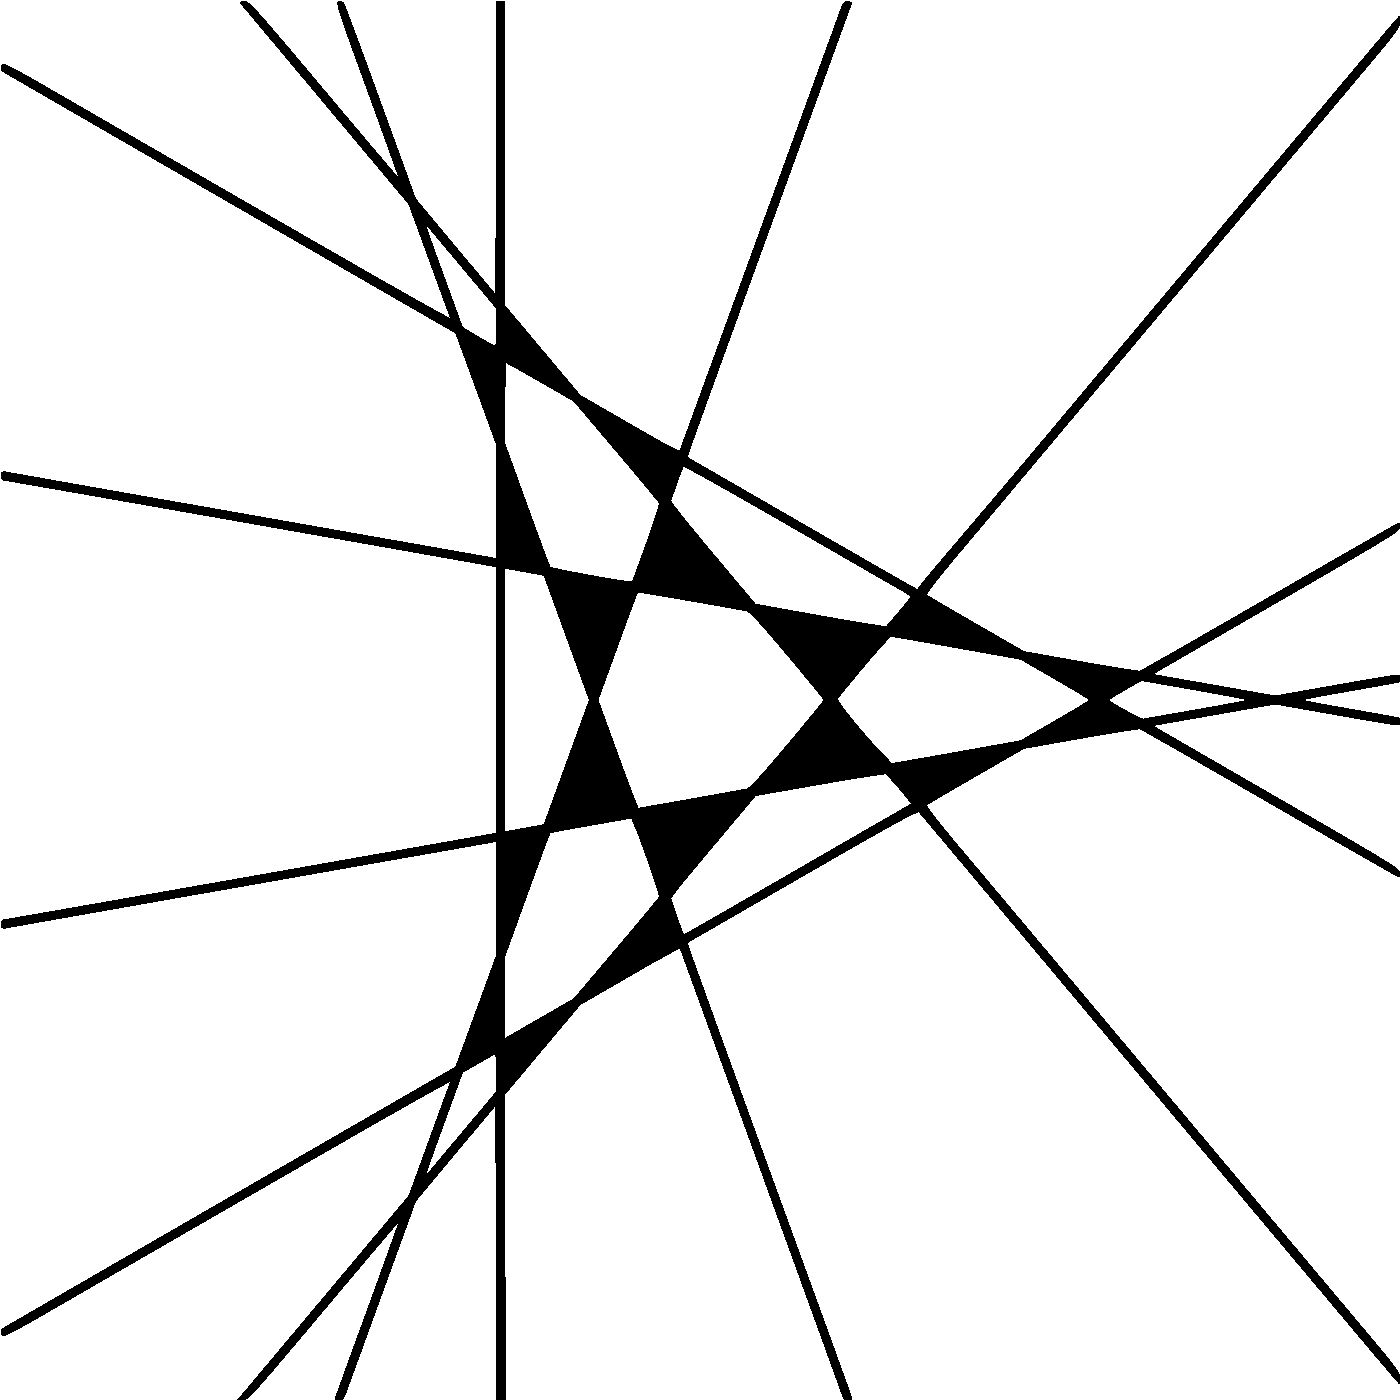
\includegraphics[height=1.5cm]{vielesing.pdf}
        &
        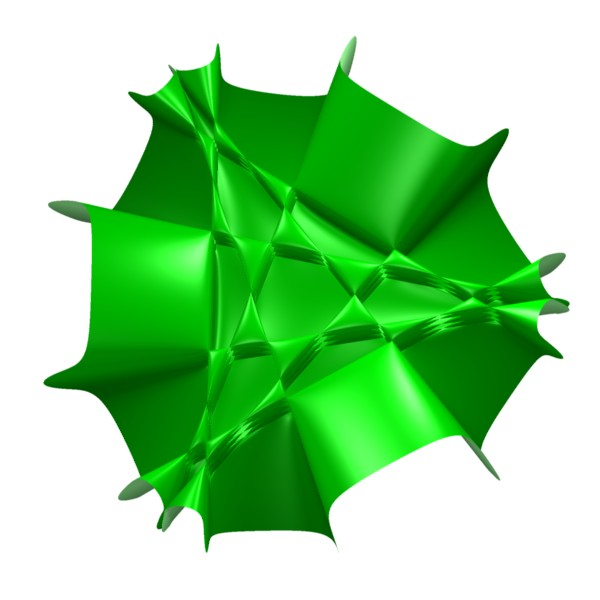
\includegraphics[height=1.5cm]{p9surface_von_oben}
      \end{tabular}
    \end{center}
\end{surferPage}
